\documentclass[12pt]{article}
\usepackage[utf8]{inputenc}
\usepackage[T1]{fontenc}
\usepackage{graphicx}
\usepackage{longtable}
\usepackage{wrapfig}
\usepackage{rotating}
\usepackage[normalem]{ulem}
\usepackage{amsmath}
\usepackage{amssymb}
\usepackage{amsthm}
\usepackage{capt-of}
\usepackage{hyperref}
\usepackage{algorithm}
\usepackage{algpseudocode}
\usepackage{minted}
\usemintedstyle{pastie}
\author{Víctor Torres}
\date{\today}
\title{Documentacion}
\setlength{\parindent}{0cm}
\hypersetup{
  colorlinks=true,
  linkcolor=blue,
  filecolor=magenta,      
  urlcolor=cyan,
  pdfauthor={Victor Torres},
  pdftitle={Documentacion},
  pdfkeywords={},
  pdfsubject={},
  pdfcreator={Victor Torres}, 
  pdflang={English}
}
\begin{document}
\thispagestyle{empty}
\begin{figure}[h!]
  \minipage{0.76\textwidth}
  
\includegraphics[height = 4.9cm ]{figures/Logo_UNAM.png}
  \label{EscudoUNAM}
  \endminipage
  \minipage{0.32\textwidth}
  
\includegraphics[height = 4.9cm ,width=4cm]{figures/Logo_FC.png}
  \label{EscudoCiencias}
  \endminipage
\end{figure}

\begin{center}
  \vspace{1cm}
  \LARGE
  UNIVERSIDAD NACIONAL AUTÓNOMA DE MÉXICO
  
  \vspace{1cm}
  \LARGE
  FACULTAD DE CIENCIAS
  
  \vspace{1.5cm}	
  \Large
  \textbf{Documentacion}
  
  \vspace{1.5cm}
  \large
  \textbf{Modelado y Programacion}
  
  \vspace{1.5cm}
  \large
  \textbf{Victor Federico Torres Trejo\\Diego Castro Rendon}
  
  \vspace{1cm}
  \today
\end{center}
\tableofcontents
\newpage

\section{Definicion del problema}
Dia a dia miles de personas van y vienen de aeropuertos a aeropuertos, cambiando drasticamente de zona horaria y clima. El aeropuerto de la Ciudad de Mexico te contrata para una tarea, la cual es entregar el informe del clima de la ciudad de salida y la ciudad de llegada para 3 mil tickets que salen el mismo dia que se corre el algoritmo.
El programa no busca que sea interactivo, ya que el mercado a quien va dirigido son sobrecargos y pilotos que desconocen de programacion, por lo que solo nos interesara el clima.
\subsection{Entender el problema}
Se quiere obtener el clima del aeropuerto de origen como el de destino, dada su longitud y latitud de cada aeropuerto ademas de una llave API para poder hacer uso de servicios web y obtener dichos datos del clima. Estos datos suficientes siempre y cuando la llave que se tenga es valida, ya que en el caso contrario no podemos solicitar el clima de ninguna ubicacion. El resultado es una solucion si la informacion que contiene es el clima de dos aeropuertos dados. Para llegar a dicho resultado nosotros al hacer la peticion tenemos que filtrar el resultado parcial para poder selccionar la informacion que mas nos interesa y proporcionar la informacion solicitada al usuario.
\subsection{Arsenal}
\begin{itemize}
\item Paradigma: orientado a objetos
\item Lenguaje: Python
\item Herramientas: API, JSON, CSV, Tkinter, DateTime
\end{itemize}

\subsection{Requisitos funcionales}
Obtener el clima de los aeropuertos de origen y destino mediante el uso de servicios web (API) dada la ubicacion de los mismos y una llave API valida..
\subsection{Requisitos no funcionales}
Garantizar la eficacia, seguridad al procesar los datos y la resistencia a fallos del programa. El programa debe ser amigable para cualquier persona ajena a los conceptos de computacion y ajena al manejo de una terminal. Debe minimizar la entrada proporcionada por el usuario.
\section{Analisis del problema}
\subsection{Proceso de Solucion}
Se va a usar tanto enfoque procedural como orientado a objetos, en cuanto al \textbf{enfoque procedural} tenemos la base de datos como entrada en formato de archivo CSV que contiene el nombre de cada ciudad, latitud y longitud del aeropuerto de destino y de origen. Leemos todos los vuelos de la base de datos y retornamos una serie de archivos JSON por cada aeropuerto de origen, que contiene el aeropuerto de origen como todos los destinos que tiene. Esto despliega todos los aeropuertos de origen disponible para que el usuario seleccione que vuelo quiere conocer, una vez que selecciona el vuelo se da como entrada el nombre del aeropuerto y despliegan todos los aeropuertos de destino dado el JSON ademas que se realiza la peticion de la informacion del aeropuerto origen.

Y despues que se despliegan los destinos el usuario selecciona uno y se le da el boton de consultar, el cual realiza la peticion del aeropuerto destino y transforma los datos JSON en datos legibles. Tambien cada consulta registramos un vuelo en el historial.

En cuanto al \textbf{enfoque orientado a objetos} se crea una clase aeropuerto que encapsula los datos de cada aeropuerto y nos permite calcular su funcion hash, esto se explicara mas adelante.

Una clase que nos permite guardar los datos de los climas para evitar realizar peticiones innecesarias, esto es cada 5 minutos pedir el clima cuando no ha cambiado en ese intervalo, tiene como atributos la lista de climas, el tamaño de dicha lista ademas de el valor de la llave API y su comportamiento es evitar esas peticiones innecesarias ademas de realizar la peticion cuando si se requiera y proporcionar el clima, para esto hace uso de la clase datosClima, la cual filtra y proporciona de una manera mas legible los datos de los clima, ya que estos al realizar una peticion nos dan en formato JSON.

Ademas tenemos una clase que nos permite hacer la filtracion o el proceso que dada la base de datos, obtener un arreglo de listas donde cada lista es un aeropuerto origen y sus aeropuertos de destino, sus atributos igual son una lista de listas y su tamaño de la lista de listas, en cuanto a comportamiento procesa cada linea del csv denominada vuelo, permite buscar si un aeropuetor de origen o destino ya existe ademas de la insercion de los de origen y escribe un archivo JSON por cada aeropuerto de origen, revisa la base de datos antes de procesarla tambien nos permite conocer los nombres de los aeropuertos de origen, esto para mostrarla en la interfaz.

Adicional tenemos una clase que codifica la clase aeropuerto para su escritura en un archivo JSON.

Y por ultimo tenemos la clase de la interfaz la cual nos permite una mejor experiencia y amigabilidad con el usuario, ya que restringe la entrada a solo validos aeropuertos y es muy intuitiva de usar, su comportamiento se define por elegir aeropuerto de origen y muestra todos los de destino, muestra todos los aeropuertos de origen, muestra los datos del clima en pantalla, permite editar la llave API, ademas de mostrar los ultimos 3 vuelos realizados

\subsection{Modelo de Datos}
Los datos se representaran principalmente a traves de tablas hash o de dispersion o diccionarios, como queremos almacenar la informacion de muchos aeropuertos se considero que un arreglo es la estructura mas adecuada para almacenar los distintos datos, esto determina el desempeño ya que el acceso a un arreglo es constante, ahora se usa una tabla de dispersion porque al tener una llave hash relacionada a los datos del aeropuerto el acceder a los valores almacenados conociendo su llave hash es tiempo constante, lo cual beneficia mucho el desempeño. Se ajusta perfecto al esbozo de una solucion ya que nos permite almacenar los datos dado un tamaño y una tabla hash, nos permite conocer y manipular la informacion de manera constante o casi constante, en el caso de lista de aeropuertos donde tenemos lista de listas, conocer la ubicacion de la lista del aeropuerto de origen es constante y generalmente no son muchos los aeropuertos de destino, por lo que acceder a ellos es muy rapido, en el caso del cache es una tabla hash la cual accedemos al clima de manera constante. Se manejan las colisiones de manera lineal, es decir, si la casilla correspondiente esta ocupada, se busca la siguiente disponible y el tamaño se selecciono tratando de minimizar las colisiones y el tamaño. No puede haber algo mejor en cuanto a tiempo porque el acceder a los datos es constante y si hay peores porque en tanto los arreglos (no hay relacion aeropuerto-indice), lista, cola, pila el acceder a los elementos es complejidad lineal.

\subsection{Seleccion de la mejor alternativa}
Ya se expuso el porque la estructura de datos tabla hash es la mejor para el proyecto y el proceso de solucion, del diseño de las clases asi como su comportamiento y atributos y el como estas interactuan entre si vistas desde un enfoque procedural, asi que solo queda como vamos a seleccionar la mejor alternativa de diseño de la interfaz, lo que se busca es minimizar la interaccion con el usuario de manera que este tenga que ingresar lo minimo indispensable para evitar errores de entrada, ya que la aplicacion va dirigida a personas ajenas a la computacion, para esto usamos el procesamiento de la base de datos para obtener los aeropuertos de origen, de esta manera podemos hacer que el usuario seleccione el aeropuerto requerido de una lista restringida, una vez seleccionada esta opcion se despliega los aeropuertos de destino de esta ciudad, al usuario seleccionar la opcion, se tiene control sobre la entrada del sistema, se evitan errores. Para poder desplegar las opciones de destino se usa tablas hash y escritura sobre archivos formato JSON, para las peticiones se sabe que no podemos hacer mas de 60 por minuto, pero tambien sabemos que el usuario no es lo suficientemente veloz como para seleccionar y consultar 60 peticiones por minuto, ademas que hay un retraso de unos segundos por la lectura del archivo JSON correspondiente para el despliegue de aeropuertos destino, por lo que eso no sera un problema, lo que si es que hay que evitar requests innecesarias por ejemplo la misma peticion con un intervalo de 10 minutos ya que el clima no ha variado significativamente, por lo que establecemos un intervalo de 30 minutos y con tablas hash simulando una memoria cache guardamos la informacion json ademas de la hora en que se ha realizado la peticion. Por ultimo para registros previos podemos visualizar los ultimos 3 vuelos registrados. Entiendase registrar por un vuelo consultado. Cabe mencionar que se va a hacer uso de OpenWeatherAPI para la request de los datos del clima de cada aeropuerto.

Para poder garantizar la minima interaccion se diseño un boceto el cual solo tiene 3 entradas: la llave API, la seleccion de aeropuerto de origen y destino la cual como ya mencionamos se acota, asi que al diseñar el boceto de la aplicacion quedo de la siguiente manera:
\newpage
\begin{figure}[h!]
  \centering
  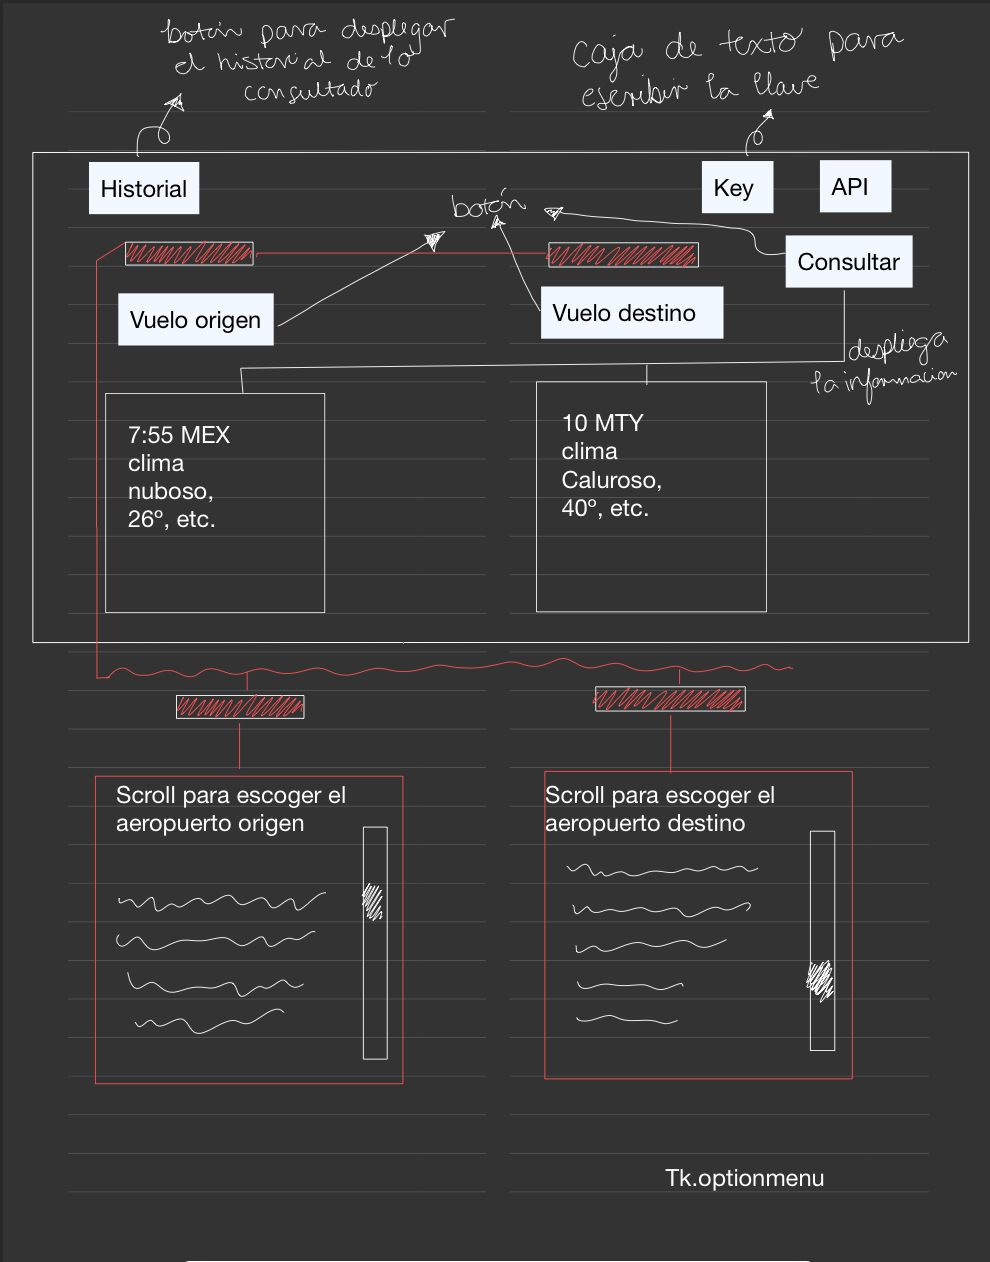
\includegraphics[scale=0.38]{figures/boceto.jpeg}
  \caption{\label{fig:label} }
\end{figure}
\newpage
\section{Pseudocodigo}
\begin{algorithmic}[1]
  \For{cada vuelo}
  \If{ciudad de origen no esta registrada}
  \State{registrala en la primera casilla vacia a partir del hash}
  \EndIf
  \If{ciudad de destino no esta registrada}
  \State{registrala en el arreglo de la ciudad de origen}
  \EndIf
  \EndFor

  
  \For{ciudad de Origen}{ciudades}
  \State{Escribir en cada json el arreglo de ciudad Origen}
  \EndFor

  
  \State{Leer ciudad Origen}
  \State{Mostrar todos los destinos posibles dada la ciudad de origen}
  \State{climaOrigen = obtenerClima(ciudadOrigen, api)}
  \State{Leer ciudad destino}
  \State{climaDestino = obtenerClima(ciudadOrigen, api)}
  \State{Mostrar Clima}
  \State{Registrar el vuelo en un archivo}

  \Function{obtenerClima}{ciudadOrigen, api}
  \If{clima ya fue registrado en cache}
  \If{Han pasado mas de 30 min desde la ultima request}
  \State{realiza una peticion y guarda en cache}
  \EndIf
  \Else
  \State{realiza la peticion}
  \State{Guarda en los datos en la primera posicion disponible}
  \EndIf
  \EndFunction
  \Function{hash}{ciudad, n}
  \State{suma = 0}
  \For{caracter}{nombre de ciudad}
  \State{suma += caracter}
  \EndFor
  \Return{(suma + abs(latitud) + abs(longitud)) \% n}
  \EndFunction
\end{algorithmic}
\section{Mantenimiento}
El sistema se dividio en 9 archivos el cual cada uno representa una clase o un conjunto de funciones para que el sistema pueda funcionar de manera correctamente, estos son:
\begin{itemize}
\item aeropuerto.py el cual encapsula los datos del aeropuerto
\item procesarArchivos.py el cual contiene las funciones para procesar la base de datos, escribir las salidas parciales en archivos JSON y leer esos archivos
\item cacheClima.py contiene la clase para simular la cache del sistema y las peticiones con la API
\item codificadorJsonAeropuerto.py la cual nos ayuda a poder transformar el aeropuerto en una salida formato JSON
\item datosClima.py la cual nos ayuda a filtrar los datos JSON en algo mas legible y facil de entender.
\item historialVuelo.py la cual nos ayuda a mantener un registro de los vuelos consultados
\item interfaz.py la cual contiene todo lo relacionado con la interfaz
\item listaDeAeropuertos.py la cual nos ayuda a procesar la base de datos usando tablas hash y guardar la informacion de cada aeropuerto de origen.
\item main.py contiene la funcion principal que es la que corre el sistema
\end{itemize}

Tambien cabe mencionar que si las librerias cambian o el mismo lenguaje recibe una actualizacion importante es importante considerar mantenimiento.
\section{Pruebas}
Como se dividio el archivo en 9 programas se haran las pruebas pertinentes a los archivos que tengan funcionalidad, en cuanto al archivo main.py es meramente declarativo, es decir solo manda a inicializar la interfaz por lo que no es necesario hacer pruebas sobre ese archivo, sobre datosClima.py como solo es utilizado para encapsular datos no tiene ningun metodo tampoco se haran pruebas sobre el, en cuanto a la interfaz sus metodos tienen entradas definidas por la misma interfaz, es decir, leer la opcion seleccionada ademas de metodos que son para mostrar informacion en pantalla o eliminarla, por lo tanto no se haran pruebas sobre interfaz.py
% codificador
\subsection{Aeropuerto}
En esta clase solo tenemos el metodo de funcion hash, por lo que probaremos con un aeropuerto cualquiera y un objeto nulo

Tenemos para el siguiente codigo un aeropuerto con la siguiente entrada tenemos que el valor hash del aeropuertoPrueba es $(77+69+88)+(10)+(100)=341\%11=3$
\begin{minted}{python}
  aeropuertoPrueba = aeropuerto.Aeropuerto('MEX', 10, 100)
  assert(aeropuertoPrueba.funcionHash(11) == 3)
\end{minted}
Por lo que al correr la siguiente salida es:
\begin{figure}[h!]
  \centering
  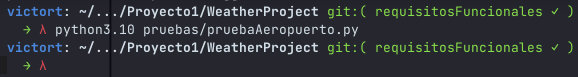
\includegraphics[scale=0.6]{pruebasPy/aeropuerto/hash1.png}
  \caption{Salida}
\end{figure}

Si ahora probamos con un resultado distinto a 3, sea 2
\begin{minted}{python}
  aeropuertoPrueba = aeropuerto.Aeropuerto('MEX', 10, 100)
  assert(aeropuertoPrueba.funcionHash(11) == 2)
\end{minted}
Se obtiene la siguiente salida:
\begin{figure}[h!]
  \centering
  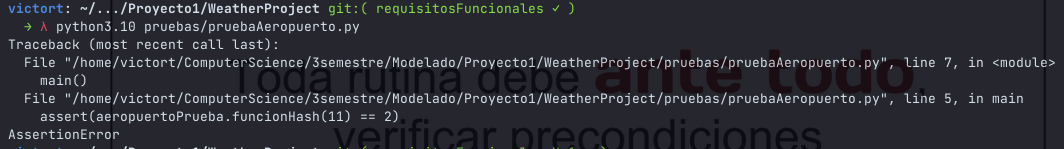
\includegraphics[scale=0.4]{pruebasPy/aeropuerto/hash2.png}
  \caption{Salida}
\end{figure}
\subsection{Prueba de Archivos}|
Para el prueba de archivos la funcion de revisarFormatoVuelo es meramente auxiliar para probar que el formato de vuelo sea de la forma: (string,string,float,float, float, float) para poder validar que el formato de vuelo es valido, pero esta funcion es llamada desde revisarCSV por lo que es redundante hacer una prueba de esto ya que se usa directamente al revisar la base de datos dada.

\subsubsection{revisarCSV}
\begin{itemize}
\item Si revisamos dataset1.csv como base de datos, la cual es una base de datos valida, tendremos la siguiente salida
\begin{minted}{python}
assert(revisarCSV('dataset1.csv')), "Base de datos invalida"
\end{minted}
  \begin{figure}[h!]
    \centering
    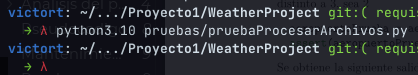
\includegraphics[scale=0.8]{pruebasPy/archivos/bien.png}
    \caption{Salida}
  \end{figure}

\item En el caso de que ingresemos datos.csv la cual es una base de datos no valida, tendremos la siguiente salida
\begin{minted}{python}
assert(revisarCSV('datosMal.csv')), "Base de datos invalida"
\end{minted}
    \begin{figure}[h!]
    \centering
    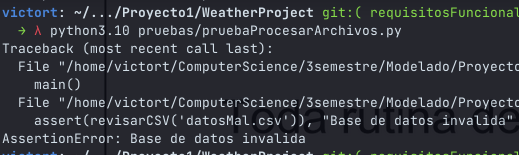
\includegraphics[scale=0.6]{pruebasPy/archivos/datosMal.png}
    \caption{Salida}
  \end{figure}

\item Si no ingresamos ningun archivo como base de datos, tendremos la siguiente salida
\begin{minted}{python}
assert(revisarCSV(None)), "Base de datos invalida"
assert(revisarCSV('')), "Base de datos invalida"
\end{minted}
    \begin{figure}[h!]
    \centering
    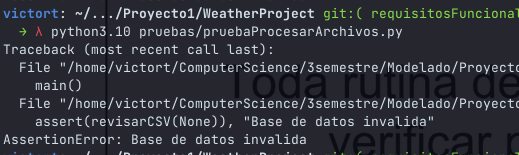
\includegraphics[scale=0.6]{pruebasPy/archivos/datosNone.png}
    \caption{Salida}
  \end{figure}
  
    \begin{figure}[h!]
    \centering
    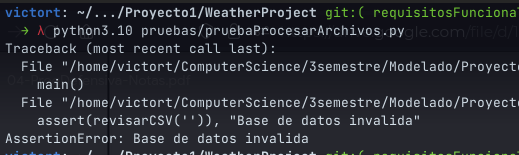
\includegraphics[scale=0.6]{pruebasPy/archivos/datosNulo.png}
    \caption{Salida}
  \end{figure}

\end{itemize}
\subsubsection{escribirDestinos}
\begin{itemize}
\item Para escribir los destinos revisaremos si le damos el archivo correcto de una base de datos recortada para poder calcular la salida, para poder comparar bien creamos una funcion auxiliar que compara dos listas
\begin{minted}{python}
lista = escribirDestinos("../pruebas/datosPrueba/baseDeDatos.csv", 2)
assert(compararLista(lista.lista, [[], [['TLC', 19.3371, -99.566]\
       , ['MTY', 25.7785, -100.107]],[]])), "Destinos invalidos"
\end{minted}
\newpage
    \begin{figure}[h!]
    \centering
    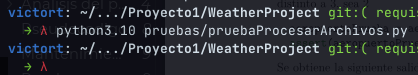
\includegraphics[scale=0.8]{pruebasPy/archivos/bien.png}
    \caption{Salida}
  \end{figure}
\item El resultado si le pasamos un archivo nulo
\begin{minted}{python}
lista = escribirDestinos("None", 2)
assert(compararLista(lista.lista, [[], [['TLC', 19.3371, -99.566]\
      , ['MTY', 25.7785, -100.107]],[]])), "Destinos invalidos"
\end{minted}
  
    \begin{figure}[h!]
    \centering
    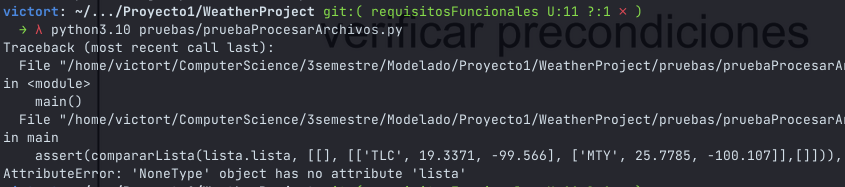
\includegraphics[scale=0.4]{pruebasPy/archivos/destinosNulo.png}
    \caption{Salida}
  \end{figure}
\end{itemize}
\subsubsection{leerDestinos}
\begin{itemize}
\item Esta funcion lee los destinos de un aeropuerto de origen, asi que se lee los destinos de Acapulco
\begin{minted}{python}
assert(leerDestinos("ACA") == [['ACA', 16.7571, -99.754],\
                                ['MEX', 19.4363, -99.0721]])
\end{minted}
  
    \begin{figure}[h!]
    \centering
    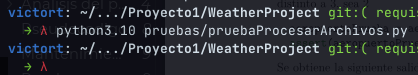
\includegraphics[scale=0.8]{pruebasPy/archivos/bien.png}
    \caption{Salida}
  \end{figure}
\item Se lee los destinos de un aeropuerto inexistente
\begin{minted}{python}
assert(leerDestinos("MEX") == [['ACA', 16.7571, -99.754],\
                                ['MEX', 19.4363, -99.0721]])
\end{minted}
  
    \begin{figure}[h!]
    \centering
    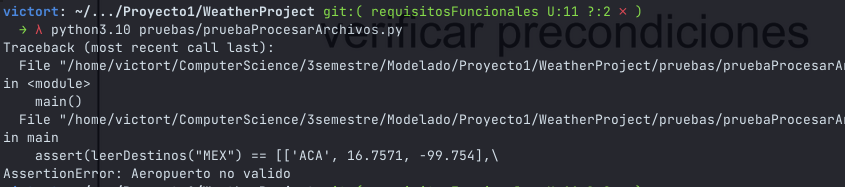
\includegraphics[scale=0.4]{pruebasPy/archivos/aeroMal.png}
    \caption{Salida}
  \end{figure}
\item Se lee los destinos de un aeropuerto nulo
\begin{minted}{python}
assert(leerDestinos(None) == [['ACA', 16.7571, -99.754],\
                                ['MEX', 19.4363, -99.0721]])
\end{minted}
  
    \begin{figure}[h!]
    \centering
    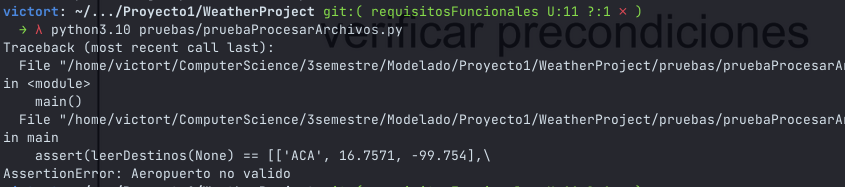
\includegraphics[scale=0.4]{pruebasPy/archivos/leerNone.png}
    \caption{Salida}
  \end{figure}
\end{itemize}
\subsection{Cache Clima}
Creamos un cache de prueba, el metodo de actualizaAPI no tiene sentido probarlo dado que solo establece un atributo, pero si lo usaremos en refrescar que realiza la peticion del servicio web
\subsubsection{refrescar}
\begin{itemize}
\item Se refresca con el aeropuerto de mexico
\begin{minted}{python}
cacheEjemplo.actualizarAPI("9d92b9e2262e46e5b34601d6f706cf43")
aeropuerto1 = Aeropuerto('MEX', 19.4363, -99.0721)
assert(cacheEjemplo.refrescarClima(aeropuerto1))\
      , "No se actualizaron los datos"
\end{minted}
  
    \begin{figure}[h!]
    \centering
    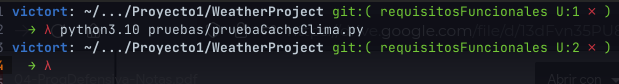
\includegraphics[scale=0.6]{pruebasPy/cache/bien.png}
    \caption{Salida}
  \end{figure}
\item Se refresca con un aeropuerto nulo
\begin{minted}{python}
cacheEjemplo.actualizarAPI("9d92b9e2262e46e5b34601d6f706cf43")
aeropuerto1 = None
assert(cacheEjemplo.refrescarClima(aeropuerto1))\
      , "No se actualizaron los datos"
\end{minted}
\begin{figure}[h!]
    \centering
    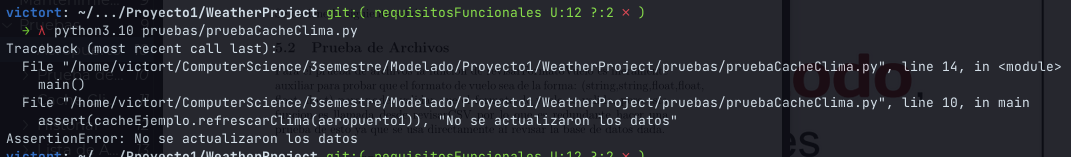
\includegraphics[scale=0.4]{pruebasPy/cache/refrescaMal.png}
    \caption{Salida}
  \end{figure}
\item No se establece una llave API por lo que es erronea la llave vacia y se solicita la informacion del aeropuerto de mexico
\begin{minted}{python}
aeropuerto1 = Aeropuerto('MEX', 19.4363, -99.0721)
assert(cacheEjemplo.refrescarClima(aeropuerto1))\
      , "No se actualizaron los datos"
\end{minted}
  \newpage
\begin{figure}[h!]
    \centering
    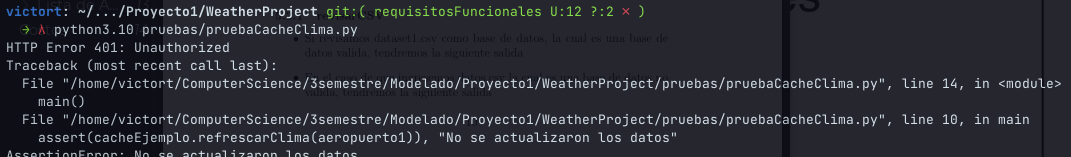
\includegraphics[scale=0.4]{pruebasPy/cache/refrescaApiMal.png}
    \caption{Salida}
  \end{figure}
\end{itemize}
\subsubsection{buscar aeropuerto}
\begin{itemize}
\item Con el aeropuerto de mexico insertado, se busca el aeropuerto de mexico
\begin{minted}{python}
aeropuerto1 = Aeropuerto('MEX', 19.4363, -99.0721)
cacheEjemplo.actualizarAPI("9d92b9e2262e46e5b34601d6f706cf43")
assert(cacheEjemplo.refrescarClima(aeropuerto1))\
      , "No se actualizaron los datos"
assert(cacheEjemplo.buscarAeropuerto(aeropuerto1) != -1)\
      , "Aeropuerto no encontrado"
\end{minted}
\begin{figure}[h!]
    \centering
    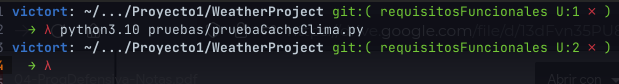
\includegraphics[scale=0.7]{pruebasPy/cache/bien.png}
    \caption{Salida}
  \end{figure}
\item Se busca el aeropuerto de acapulco el cual no se encuentra en el cache
\begin{minted}{python}
aeropuerto1 = Aeropuerto('MEX', 19.4363, -99.0721)
aeropuerto2 = Aeropuerto('ACA', 16.7571, -99.754)
cacheEjemplo.actualizarAPI("9d92b9e2262e46e5b34601d6f706cf43")
assert(cacheEjemplo.refrescarClima(aeropuerto1))\
      , "No se actualizaron los datos"
assert(cacheEjemplo.buscarAeropuerto(aeropuerto1) != -1)\
      , "Aeropuerto no encontrado"
\end{minted}
  \newpage
 \begin{figure}[h!]
    \centering
    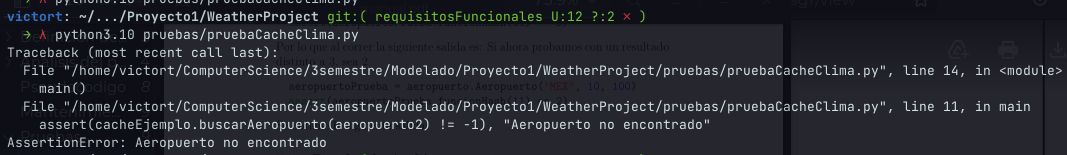
\includegraphics[scale=0.4]{pruebasPy/cache/aeroNoEncontrado.png}
    \caption{Salida}
  \end{figure}
\item Se busca un aeropuerto nulo
\begin{minted}{python}
aeropuerto1 = Aeropuerto('MEX', 19.4363, -99.0721)
cacheEjemplo.actualizarAPI("9d92b9e2262e46e5b34601d6f706cf43")
assert(cacheEjemplo.refrescarClima(aeropuerto1))\
      , "No se actualizaron los datos"
assert(cacheEjemplo.buscarAeropuerto(None) != -1)\
      , "Aeropuerto no encontrado"
\end{minted}
  \begin{figure}[h!]
    \centering
    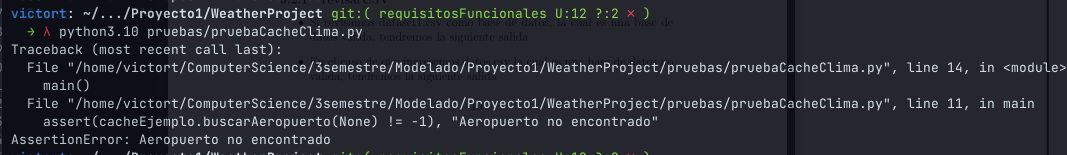
\includegraphics[scale=0.4]{pruebasPy/cache/buscaNone.png}
    \caption{Salida}
  \end{figure}
\end{itemize}
\subsubsection{obtener clima y realizar peticion}
Se compara con realizar peticion ya que los datos que hay en el cache son formato JSON que son los datos que devuelve realizar peticion pero realizar peticion lo hace directamente.
\begin{itemize}
\item Se obtiene el clima de un aeropuerto que ya se refresco el aeropuerto
\begin{minted}{python}
aeropuerto1 = Aeropuerto('MEX', 19.4363, -99.0721)
cacheEjemplo.actualizarAPI("9d92b9e2262e46e5b34601d6f706cf43")
assert(cacheEjemplo.refrescarClima(aeropuerto1))\
      , "No se actualizaron los datos"
assert(cacheEjemplo.obtenerClima(aeropuerto1)\
       .__eq__(DatosClima(cacheEjemplo\
       .realizarPeticion(aeropuerto1)))), "Datos JSON distintos"
\end{minted}
 \begin{figure}[h!]
    \centering
    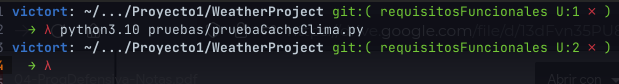
\includegraphics[scale=0.6]{pruebasPy/cache/bien.png}
    \caption{Salida}
  \end{figure}
\item Se busca el clima de un aeropuerto nulo
\begin{minted}{python}
aeropuerto1 = Aeropuerto('MEX', 19.4363, -99.0721)
cacheEjemplo.actualizarAPI("9d92b9e2262e46e5b34601d6f706cf43")
assert(cacheEjemplo.refrescarClima(aeropuerto1))\
      , "No se actualizaron los datos"
assert(cacheEjemplo.obtenerClima(None)\
       .__eq__(DatosClima(cacheEjemplo\
       .realizarPeticion(aeropuerto1)))), "Datos JSON distintos"
\end{minted}
\begin{figure}[h!]
    \centering
    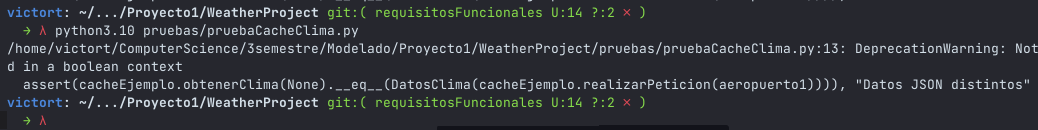
\includegraphics[scale=0.4]{pruebasPy/cache/obtenNone.png}
    \caption{Salida}
  \end{figure}
\item Se busca el clima de un aeropuerto que no esta en el cache
\begin{minted}{python}
aeropuerto1 = Aeropuerto('MEX', 19.4363, -99.0721)
cacheEjemplo.actualizarAPI("9d92b9e2262e46e5b34601d6f706cf43")
assert(cacheEjemplo.refrescarClima(aeropuerto1))\
       , "No se actualizaron los datos"
assert(cacheEjemplo.obtenerClima(aeropuerto2)\
       .__eq__(DatosClima(cacheEjemplo\
       .realizarPeticion(aeropuerto1)))), "Datos JSON distintos"
\end{minted}
  \newpage
 \begin{figure}[h!]
    \centering
    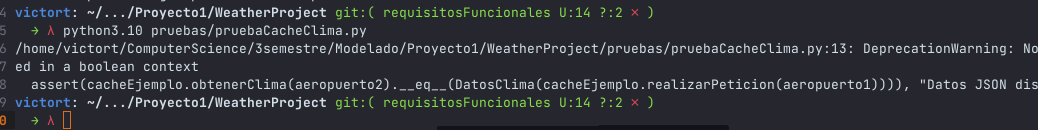
\includegraphics[scale=0.4]{pruebasPy/cache/obtenInex.png}
    \caption{Salida}
  \end{figure}
\item Por ultimo se prueba realizar peticion para un aeropuerto nulo
\begin{minted}{python}
aeropuerto1 = Aeropuerto('MEX', 19.4363, -99.0721)
cacheEjemplo.actualizarAPI("9d92b9e2262e46e5b34601d6f706cf43")
assert(cacheEjemplo.refrescarClima(aeropuerto1))\
       , "No se actualizaron los datos"
assert(cacheEjemplo.realizarPeticion(None) != None)\
      , "Datos JSON nulos"
\end{minted}
\begin{figure}[h!]
    \centering
    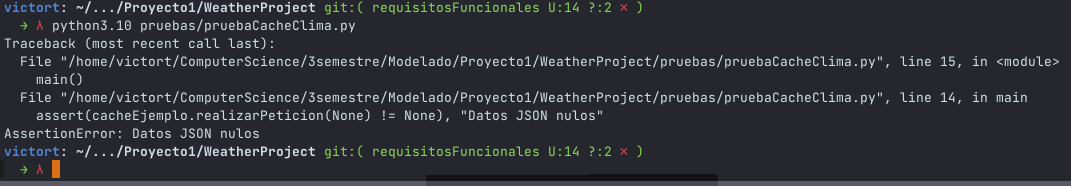
\includegraphics[scale=0.4]{pruebasPy/cache/pideNone.png}
    \caption{Salida}
  \end{figure}
\end{itemize}
\subsection{Historial}
\subsubsection{Obtener numero de vuelo}
Se busca que devuelva un dato de tipo entero
\begin{minted}{python}
assert(type(obtenerNumeroDeVuelo()) == int)\
       , "Tipo de dato incorrecto"
\end{minted}
\begin{figure}[h!]
    \centering
    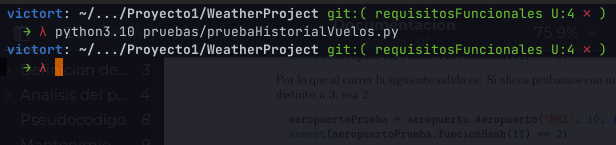
\includegraphics[scale=0.7]{pruebasPy/historial/bien.png}
    \caption{Salida}
  \end{figure}
Solo se realizo una prueba porque la funcion es sin parametros, salida:
\subsubsection{Convertir a vuelo}
Usaremos un objeto de la clase clima cache para poder acceder a la funcion de realizar peticion, ya que esta funcion toma datos JSON y los convierte en texto legible para vuelos
\begin{itemize}
\item Revisamos que lo que nos devuelva es una string ya que quiere decir que proceso bien los datos JSON de entrada.
\begin{minted}{python}
aeropuerto1 = Aeropuerto('MEX', 19.4363, -99.0721)
cacheClima = CacheClima(11)
cacheClima.actualizarAPI("9d92b9e2262e46e5b34601d6f706cf43")
cacheClima.refrescarClima(aeropuerto1)
assert(type (convertirAVuelo(\
            cacheClima.realizarPeticion(aeropuerto1),\
            cacheClima.realizarPeticion(aeropuerto1))) == str)
\end{minted}
\begin{figure}[h!]
    \centering
    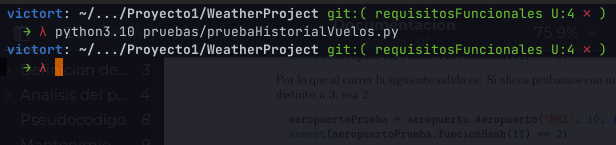
\includegraphics[scale=0.7]{pruebasPy/historial/bien.png}
    \caption{Salida}
  \end{figure}
\item Se le manda dos datos nulos como ambos parametros

\begin{minted}{python}
assert(type (convertirAVuelo(cacheClima.obtenerClima(None),\
                             cacheClima.obtenerClima(None))) == str)
\end{minted}
  En ambos caso tenemos la misma salida, una string que representa el vuelo
\end{itemize}
\subsection{Lista de Aeropuertos}
\subsubsection{Procesar Vuelo}
\begin{itemize}
\item Se revisa que si se procesa un vuelo de acapulco a mexico, se inserta de manera correcta en la lista de listas.
\begin{minted}{python}
vuelo = ['ACA', 'MEX', 16.7571, -99.754, 19.4363, -99.0721]
assert(listaPrueba.procesarVuelo(vuelo) != -1)    
\end{minted}
\begin{figure}[h!]
    \centering
    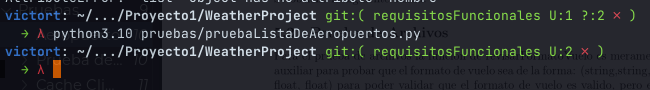
\includegraphics[scale=0.7]{pruebasPy/listaAeropuertos/bien.png}
    \caption{Salida}
  \end{figure}
\item Se revisa si se procesa un vuelo nulo
\begin{minted}{python}
vuelo = None
assert(listaPrueba.procesarVuelo(vuelo) != -1)    
\end{minted}

\begin{figure}[h!]
    \centering
    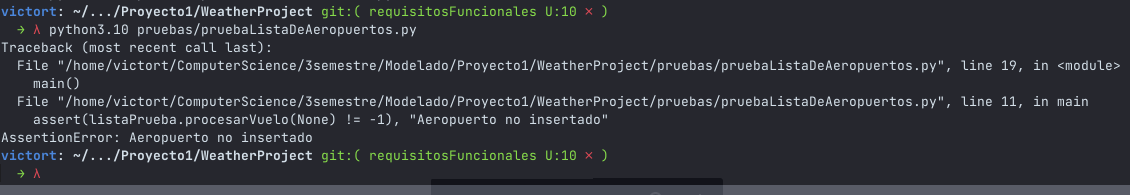
\includegraphics[scale=0.3]{pruebasPy/listaAeropuertos/procesaNone.png}
    \caption{Salida}
  \end{figure}
\end{itemize}
\subsubsection{Buscar Aeropuerto de Origen}
Se toma el vuelo registrado de acapulco a mexico
\begin{itemize}
\item Si se proceso el vuelo de acapulco a mexico, se busca a acapulco dentro de la lista
\begin{minted}{python}
aeropuerto1 = Aeropuerto('ACA', 16.7571, -99.754)
assert(listaPrueba.buscarAeropuertoOrigen(aeropuerto1) != -1)    
\end{minted}
\begin{figure}[h!]
    \centering
    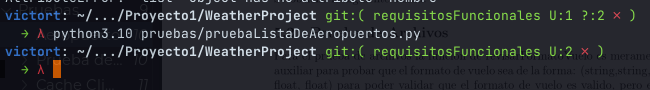
\includegraphics[scale=0.7]{pruebasPy/listaAeropuertos/bien.png}
    \caption{Salida}
\end{figure}

\item Se busca un aeropuerto nulo
\begin{minted}{python}
aeropuerto1 = Aeropuerto('ACA', 16.7571, -99.754)
assert(listaPrueba.buscarAeropuertoOrigen(None) != -1)    
\end{minted}
\begin{figure}[h!]
    \centering
    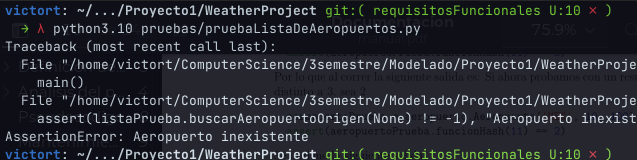
\includegraphics[scale=0.4]{pruebasPy/listaAeropuertos/buscaNone.png}
    \caption{Salida}
  \end{figure}

\item Se busca un aeropuerto de un vuelo que no hemos procesado
\begin{minted}{python}
aeropuertoPrueba = Aeropuerto('MTY', 0 ,0)
assert(listaPrueba.buscarAeropuertoOrigen(aeropuertoPrueba) != -1)    
\end{minted}
\begin{figure}[h!]
    \centering
    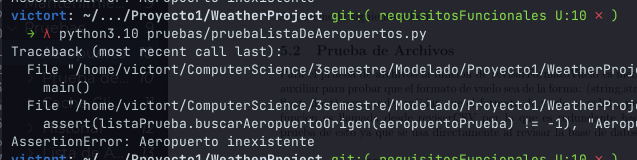
\includegraphics[scale=0.7]{pruebasPy/listaAeropuertos/buscaInex.png}
    \caption{Salida}
  \end{figure}
\end{itemize}
\subsubsection{Insertar aeropuerto de origen}
\begin{itemize}
\item Dado un aeropuerto de origen se busca que se haya insertado en un indice valido
\begin{minted}{python}
assert(listaPrueba.insertarAeropuertoOrigen(aeropuertoPrueba) != -1)\
       , "No se inserto el aeropuerto"
\end{minted}
\begin{figure}[h!]
    \centering
    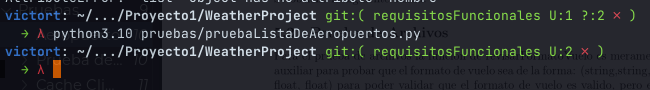
\includegraphics[scale=0.6]{pruebasPy/listaAeropuertos/bien.png}
    \caption{Salida}
  \end{figure}
\item Se inserta un aeropuerto nulo
\begin{minted}{python}
assert(listaPrueba.insertarAeropuertoOrigen(None) != -1)\
      , "No se inserto el aeropuerto"
\end{minted}
\begin{figure}[h!]
    \centering
    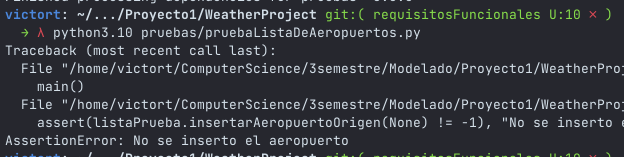
\includegraphics[scale=0.6]{pruebasPy/listaAeropuertos/insertaNone.png}
    \caption{Salida}
  \end{figure}
\end{itemize}
\subsubsection{Buscar aeropuerto de destino}
Se usa la misma lista con el vuelo de acapulco a mexico
\begin{itemize}
\item Dado el vuelo anterior de acapulco a mexico se busca a mexico dentro de la lista correspondiente a acapulco
\begin{minted}{python}
assert(listaPrueba.buscarAeropuertoDestino(\
       listaPrueba.lista[aeropuerto1.funcionHash(11)]\
       , aeropuerto2.nombre)), "Aeropuerto inexistente"
\end{minted}
\begin{figure}[h!]
    \centering
    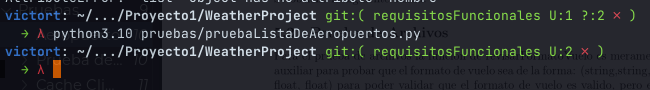
\includegraphics[scale=0.6]{pruebasPy/listaAeropuertos/bien.png}
    \caption{Salida}
  \end{figure}

\item Se busca un aeropuerto nulo en la lista de acapulco
\begin{minted}{python}
assert(listaPrueba.buscarAeropuertoDestino(\
       listaPrueba.lista[aeropuerto1.funcionHash(11)]\
      , None)), "Aeropuerto inexistente"
\end{minted}
\begin{figure}[h!]
    \centering
    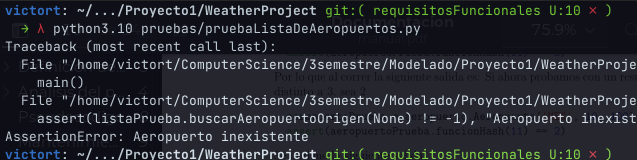
\includegraphics[scale=0.6]{pruebasPy/listaAeropuertos/buscaNone.png}
    \caption{Salida}
  \end{figure}
\item Se busca un aeropuerto en una lista vacia
\begin{minted}{python}
assert(listaPrueba.buscarAeropuertoDestino([], aeropuerto2.nombre))\
       , "Aeropuerto inexistente"
\end{minted}
\begin{figure}[h!]
    \centering
    \includegraphics[scale=0.6]{pruebasPy/listaAeropuertos/buscaDvacio.png}
    \caption{Salida}
  \end{figure}
\end{itemize}
\subsubsection{Revisar archivos}
Se revisa que se hayan escrito los aeropuertos de manera correcta de acuerdo a los nombres de aeropuerto
\begin{minted}{python}
assert(listaPrueba.revisarArchivosJSON()), "JSONs no escritos"
\end{minted}
\begin{figure}[h!]
    \centering
    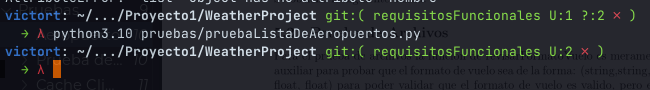
\includegraphics[scale=0.6]{pruebasPy/listaAeropuertos/bien.png}
    \caption{Salida}
  \end{figure}

\subsubsection{Obtener nombres}
Si solo se han insertado acapulco y monterrey como aeropuertos de origen se busca que se devuelvan solo los nombres de esos dos aeropuertos
\begin{minted}{python}
assert(listaPrueba.obtenerNombres() == ['ACA', 'MTY'])
\end{minted}
\begin{figure}[h!]
    \centering
    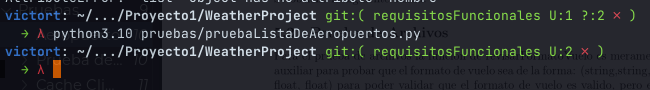
\includegraphics[scale=0.6]{pruebasPy/listaAeropuertos/bien.png}
    \caption{Salida}
  \end{figure}

\section{Costos}
El costo de desarrollo por la beta seria de \$1000, el de desarrollo final seria un costo total ya de \$2000 y por darle mantenimiento habria un costo de \$500.
\end{document}

%%% Local Variables:
%%% mode: latex
%%% TeX-master: t
%%% End:
